\section{\hspace{1em}Въведение}
\begin{frame}[t]{Комари}
  \begin{figure}[h]
    \centering
    \begin{subfigure}{0.5\textwidth}
      \centering
      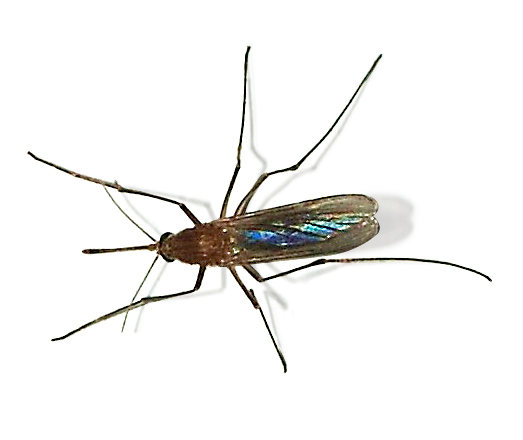
\includegraphics[width=0.5\textwidth]{Culex_pipiens_2007-1.jpg}
      \caption{\textit{Culex pipiens}}
      \label{fig:Culex}
    \end{subfigure}%
    \begin{subfigure}{0.5\textwidth}
      \centering
      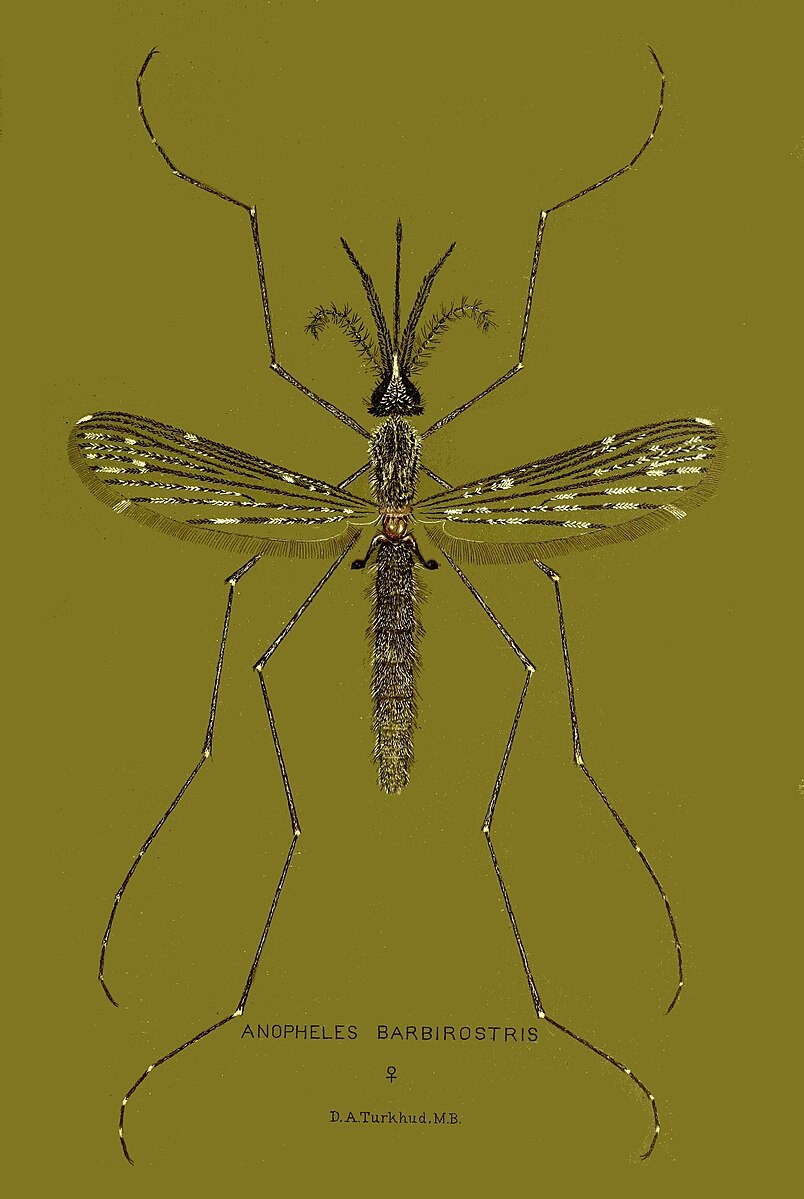
\includegraphics[width=0.5\textwidth]{Anopheles_barbirostris.jpg}
      \caption{\textit{Anopheles barbirostris}}
      \label{fig:Anopheles}
    \end{subfigure}
  \end{figure}
\end{frame}

\begin{frame}[t]{Термини от епидемологията}
  \begin{itemize}
    \item Патоген е причинител на зараза (напр. вирус, бактерия, прион).
    \item Вектор е носител на патоген, който може да зарази други индивиди.
    \item S (Susceptible) - податливи са тези, които не носят патогена и могат да бъдат заразени с него
    \item E (Exposed) - латентни са носители на патогена, които не могат да го предадат
    \item I (Infectious) - заразни са носители на патогена, които могат да го предадат
    \item R (Removed/Recovered/Resistant) - резистентни са тези, които имат (или са получили след заразяване с патогена) имунитет (може да е временен) към патогена и не могат нито да го разпространят, нито да бъдат заразени
  \end{itemize}
\end{frame}

\begin{frame}[t]{Развитие на заразата}
  В зависимост от природата на заразата, могат да се наблюдават различни преходи на индивид от един в друг клас с течение на времето:
  \begin{itemize}
    \item $S \rightarrow E \rightarrow I \rightarrow R \rightarrow S$ (SEIRS)
    \item $S \rightarrow I \rightarrow R$ (SIR) напр. рубеола
    \item $S \rightarrow I \rightarrow R \rightarrow S$ (SIRS)
    \item $S \rightarrow E \rightarrow I$ (SEI) напр. HIV
    \item $S \rightarrow I \rightarrow S$ (SIS) напр. малария, инфлуенца
  \end{itemize}
  Понякога по-сложни заболявания могат да се моделират с по-прости модели (напр. да допуснем, че няма латентна фаза), но тогава няма да получим същата точност при прогноза на развитието на заболяването.
\end{frame}

\begin{frame}[t]{Разпространение на заразата}
  Kатегориите влияят една на друга, например заразните могат да заразят човек от податливите и така той да се причисли към тяхната група.

  Възможно е да имаме повече от една съвкупност от групи SEIRS хора (напр. разделение по възраст, местообитание), за които да имаме различни податливости на патогена.

  Възможно е да имаме повече от една съвкупност от групи SEIRS, отговаряща за различни видове.

  Възможно е да се разглежда популационната динамика при развитие за прогнози далеч във времето.
\end{frame}

\begin{frame}[t]{Малария}
  Патогенът е един от няколко маларийни плазмодии (едноклетъчни еукариоти, т.е. едноклетъчни с ядро).

  Симптоми са периодичен пароксизъм(продължителни спазми, потене, треска), умора, главоболие, белодробен оток, разрастнал се черен дроб, смърт. Различават се по интензивност спрямо вида плазмодий.

  През XIX са открили връзката с болестта и присъствието на комари, но първоначално се е предполагало, че патогена се пренася по вода.

  В днешно време се среща основно в Африка, Югоизточна Азия.

  Разпространява се чрез ухапването на женските комари от род \textit{Anopheles}.
\end{frame}

\begin{frame}[t]{Малариен плазмодий}
  \begin{figure}
    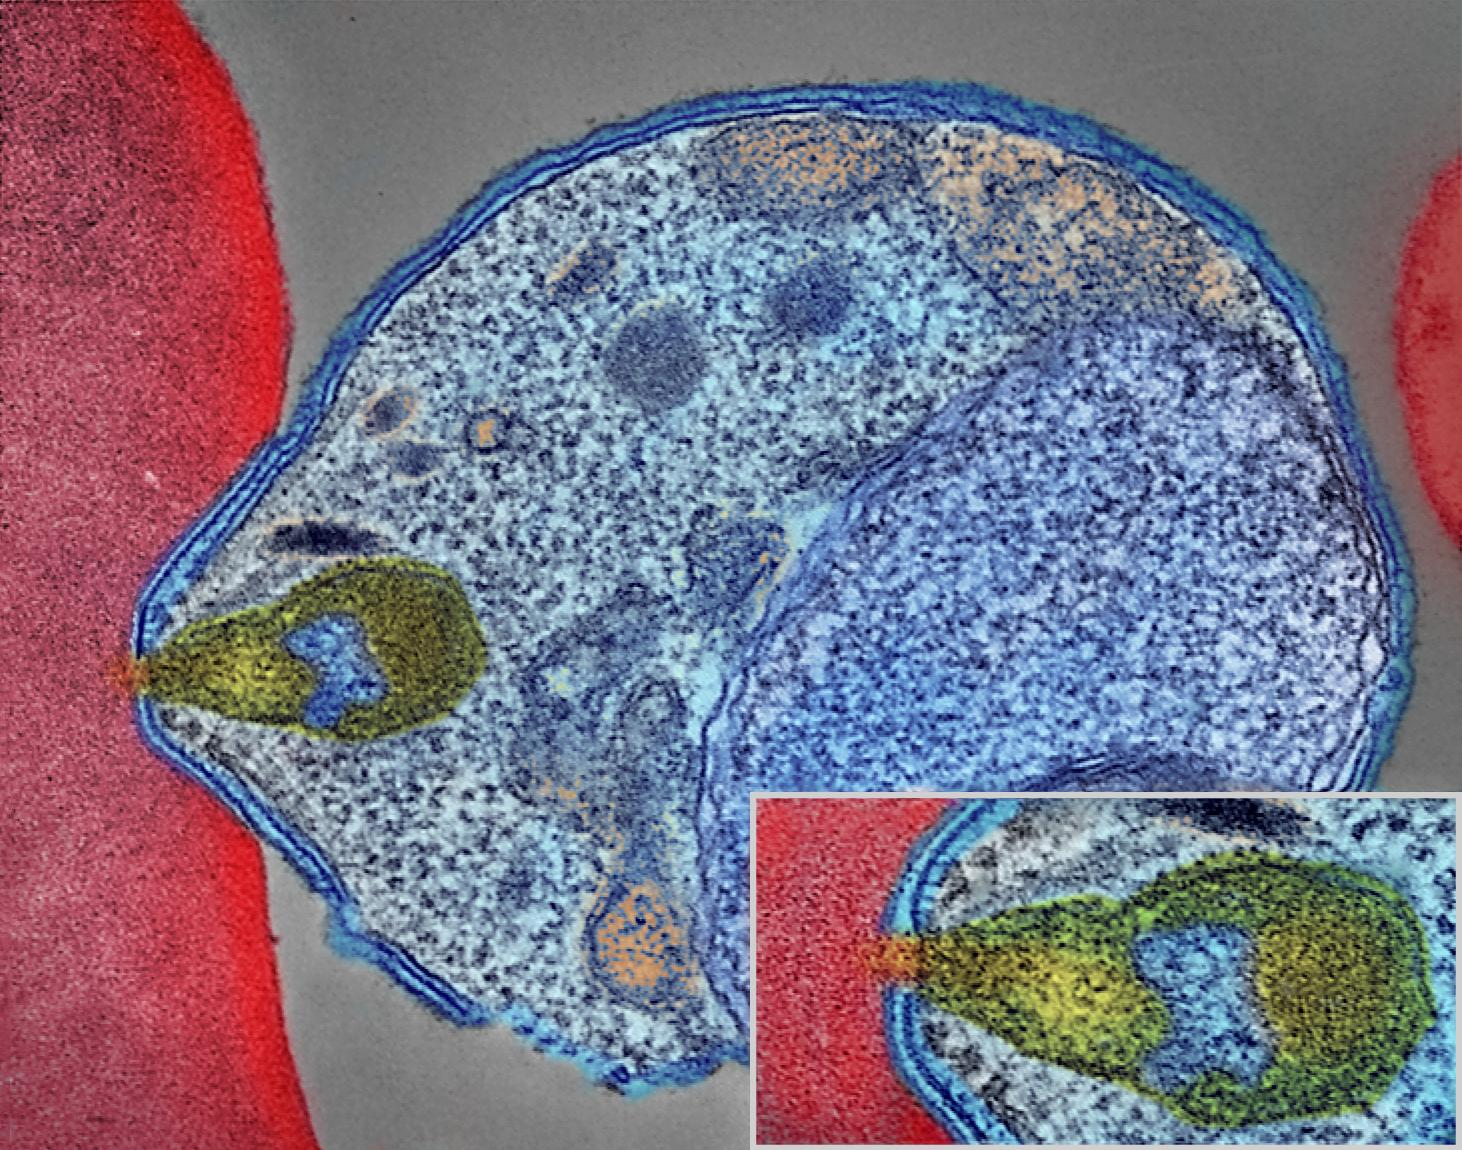
\includegraphics[height=0.6\textheight]{Malaria_Parasite_Connecting_to_Human_Red_Blood_Cell_(34034143483).jpg}
    \centering
    \caption{Оцветена електронно микроскопска снимка на плазмодий нападащ еритроцит}
  \end{figure}
\end{frame}

\begin{frame}[t]{Малариен плазмодий}
  \begin{figure}
    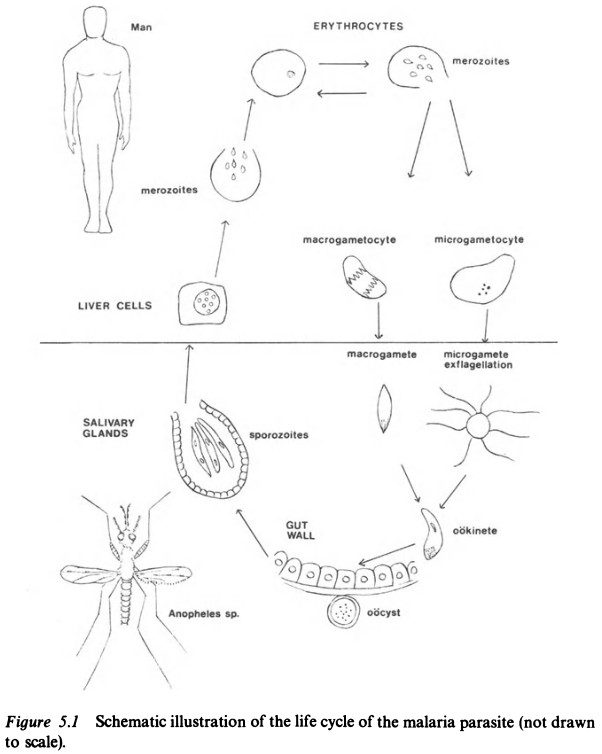
\includegraphics[height=0.75\textheight]{malaria-transmission.png}
    \centering
    \caption{Жизнен цикъл на патогена}
  \end{figure}
\end{frame}
